\documentclass[10pt]{article}
\setlength{\parskip}{\baselineskip}
\usepackage{fullpage}
\usepackage{csquotes}
\usepackage{graphicx}
\usepackage{amsmath,amsfonts,amssymb}

\title{Homework 5}
\author{CSCI 4511W Spring 2018}
\begin{document}
\date{April 25, 2018}
\maketitle

Instructor: Dr.Maria Gini\hfill Joowon Kim(kimx4342)

\hrulefill

\begin{enumerate}
\item You are given a train engine and three boxcars, which are all at the Chicago train station. There are two boxcars in Milwaukee. There is a train track connecting Minneapolis to Milwaukee, and one connecting Milwaukee to Chicago. 
Your goal is to couple the five boxcars with the engine, move them all to Minneapolis, and take the engine back to Chicago. 
You can couple a boxcar with an engine if they are both at the same train station. You can couple one boxcar at a time with an engine. You can connect as many boxcars as you want to an engine. Boxcars can be moved only if coupled with an engine. An engine can move from a station to another as long as there is a track connecting the stations, either directly or indirectly through another city. 
Answer the following questions: \newline
\newline
Predicate: \newline
\newline
 Boxcar(a) : boxcar $a$. \newline
 Engine(a) : engine $a$. \newline
 At(a, x) : $a$ is at location $x$. \newline
 Coupled(a, c) : $a$ is coupled with $c$. \newline
 Connected(y, t): $y$ is connected to $t$. \newline
 Station(a) : station $a$. \newline

\begin{enumerate}
\item Define the action schemas for this train domain. Provide a description of the predicates you use sufficient to understand them unequivocally. \newline
$\rightarrow$ \newline
Action(Couple(b, e, s), \newline
\hspace*{1.0cm} PRECOND: At(b, s) $\wedge$ At(e, s) $\wedge$ Boxcar(b) $\wedge$ Engine(e) $\wedge$ Station(s) \newline
\hspace*{1.0cm} EFFFECT: Coupled(b, e)) \newline
\newline
Action(MoveT($b_1$...$b_n$, e, $s_1$, $s_2$), \newline
\hspace*{1.0cm} PRECOND: Boxcar($b_1$) $\wedge$ ... $\wedge$ Boxcar($b_n$) $\wedge$ Engine(e) $\wedge$ Station($s_1$) $\wedge$ Station($s_2$) $\wedge$ At($b_1, s_1$) $\wedge$ ...  $\wedge$ At($b_n, s_1$) $\wedge$ At(e, $s_1$) $\wedge$ Coupled($b_1$, e) $\wedge$ ... Coupled($b_n$, e) $\wedge$ Connected($s_1$, $s_2$) \newline
\hspace*{1.0cm} EFFECT: $\neg$ At($b_1$, $s_1$) $\wedge$ ... $\wedge$ $\neg$ At($b_n$, $s_1$) $\wedge$ $\neg$ At(e, $s_1$) $\wedge$ At($b_1$, $s_2$) $\wedge$ ... $\wedge$ At($b_n$, $s_2$) $\wedge$ At(e, $s_2$)) \newline
\newline
Action(MoveE(e,$s_1$,$s_2$), \newline
\hspace*{1.0cm} PRECOND: Engine(e) $\wedge$ Station($s_1$) $\wedge$ Station($s_2$) $\wedge$ At(e,$s_1$) $\wedge$ Connected($s_1$, $s_2$) \newline
\hspace*{1.0cm} EFFECT: $\neg$At(e, $s_1$) $\wedge$ At(e, $s_2$)) \newline
\newline
Action($\neg$Coupled(b,e,s), \newline
\hspace*{1.0cm} PRECOND: Boxcar(b) $\wedge$ Engine(e) $\wedge$ Station(s) $\wedge$ At(b,s) $\wedge$ At(e,s) $\wedge$ Coupled(b,e) \newline
\hspace*{1.0cm} $\neg$Coupled(b,e)) \newline

\item Define the initial state and the goal state. \newline
$\rightarrow$ \newline
Initial State : \newline
(Boxcar($B_1$) $\wedge$ Boxcar($B_2$) $\wedge$ Boxcar($B_3$) $\wedge$ Boxcar($B_4$) $\wedge$ Boxcar($B_5$)) $\wedge$ (Station(Chicago) $\wedge$ Station(Minneapolis) $\wedge$ Station(Milwaukee)) $\wedge$ Engine(E) $\wedge$ At($B_1$, Chicago) $\wedge$ At($B_2$, Chicago) $\wedge$ At($B_3$, Chicago) $\wedge$ At(E, Chicago) $\wedge$ At($B_4$, Milwaukee) $\wedge$ At($B_5$, Milwaukee) $\wedge$ Connected(Minneapolis, Milwaukee) $\wedge$ Connected(Milwaukee, Chicago) \newline

Goal State: \newline
At($B_1$, Minneapolis) $\wedge$ At($B_2$, Minneapolis) $\wedge$ At($B_3$, Minneapolis) $\wedge$ At($B_4$, Minneapolis) $\wedge$ At($B_5$, Minneapolis) $\wedge$ At(E, Chicago) \newline
\item Show a plan that can be obtained using your action schemas to accomplish the goal. \newline
$\rightarrow$ \newline
Couple($B_1$,Engine,Chicago), Couple($B_2$,Engine,Chicago), Couple($B_3$,Engine,Chicago), \newline MoveT($B_1,B_2,B_3$,Engine,Chicago,Milwaukee), \newline Couple($B_4$,Engine,Milwaukee), Couple($B_5$,Engine,Milwaukee), \newline MoveT($B_1,B_2,B_3,B_4,B_5$,Engine,Milwaukee,Minneapolis), \newline $\neg$Coupled($B_1$,Engine,Minneapolis), $\neg$Coupled($B_2$,Engine,Minneapolis), $\neg$Coupled($B_3$,Engine,Minneapolis), $\neg$Coupled($B_4$,Engine,Minneapolis), $\neg$Coupled($B_5$,Engine,Minneapolis), \newline MoveE(Engine,Minneapolis,Milwaukee), MoveE(Engine,Milwaukee,Chicago)
\end{enumerate}
\item Consider the following variation to the block stacking domain; blocks are arranged on a table in $N^2$ locations corresponding to the cells of a N x N grid. At most one block can be located in any given location and no more than H blocks can be stacked. \newline
\newline
Predicate: \newline
\newline
On(x,y,h) : block $x$ is on block $y$ at height $h$. ($h \leq H$) \newline
In(x,l) : block $x$ is at $l$ \newline
Block(x) : block $x$ \newline
Location(l) : Location $l$ in $N * N$ \newline
NotOn(x) : Nothing on $x$ \newline
\begin{enumerate}
\item Define action schemas for moving blocks between locations, between blocks, and between locations and blocks. Define the predicates you use and make sure the notation you use for writing the schemas is clearly defined. \newline
$\rightarrow$ \newline
Action(MoveLocToLoc(x,$l_1$,$l_2$) \newline
\hspace*{1.0cm} PRECOND: Block(x) $\wedge$ Location($l_1$) $\wedge$ Location($l_2$) $\wedge$ In(x,$l_1$) $\wedge$ NotOn(x) $\wedge$ NotOn($l_2$) $\wedge$ (h $\leq$ H) \newline
\hspace*{1.0cm} EFFECT: $\neg$In(x,$l_1$) $\wedge$ In(x,$l_2$) $\wedge$ NotOn($l_1$) $\wedge$ $\neg$NotOn($l_2$)) \newline
\newline
Action(MoveBlockToBlock(x,$x_1$,$x_2$,$h_1$,$h_2$) \newline
\hspace*{1.0cm} PRECOND: Block(x) $\wedge$ Block($x_1$) $\wedge$ Block($x_2$) $\wedge$ On(x,$x_1$,$h_1$) $\wedge$ NotOn(x) $\wedge$ NotOn($x_2$) $\wedge$ ($h_1$ $\leq$ H) $\wedge$ ($h_2$ $\leq$ H) \newline
\hspace*{1.0cm} EFFECT: $\neg$On(x,$x_1$) $\wedge$ On(x,$x_1$,h) $\wedge$ NotOn(l) $\wedge$ $\neg$NotOn($x_2$)) \newline
\newline
Action(MoveBlockToLoc(x,$x_1$,l,h) \newline
\hspace*{1.0cm} PRECOND: Block(x) $\wedge$ Block($x_1$) $\wedge$ Location(l) $\wedge$ On(x,$x_1$,h) $\wedge$ NotOn(b) $\wedge$ NotOn(l) $\wedge$ (h $\leq$ H) \newline
\hspace*{1.0cm} EFFECT: $\neg$On(x,$x_1$,h) $\wedge$ In(x,l) $\wedge$ NotOn($x_1$) $\wedge$ $\neg$NotOn(l)) \newline
\newline
Action(MoveLocToBlock(x,l,$x_2$,h) \newline
\hspace*{1.0cm} PRECOND: Block(x) $\wedge$ Block($x_2$) $\wedge$ Location(l) $\wedge$ In(x,l) $\wedge$ NotOn(x) $\wedge$ NotOn($x_2$) $\wedge$ (h $\leq$ H) \newline
\hspace*{1.0cm} EFFECT: $\neg$In(x,l) $\wedge$ On(x,$x_2$,h) $\wedge$ NotOn(l) $\wedge$ $neg$NotOn($x_2$)) \newline
\item Assume the initial state and goal state are completely specified (i.e. you know where each block is), and assume the number of blocks is less or equal to $N^2$. Propose a trivial algorithm (not a planning algorithm) for solving any problem in this domain. \newline
$\rightarrow$ \newline
We assumed that initial state and goal state are completely specified. First, the algorithm would take the initial state and make it node. Than, it would take actions that can be applied to the initial state. By doing action, if result state comes out, make it new node and append to initial node. Than, repeat the same thing from the child nodes. After all of these process are done, use the depth-first search and if the goal states comes out, return path and this would be the solution for it. \newline
\item Is your algorithm guaranteed to find an optimal solution in terms of number of steps? \newline
$\rightarrow$ \newline
No, this algorithm would not guaranteed to have optimal solution. Because we cannot say that the solution that is first found is optimal. It can have more steps compare to the optimal solution of tree. \newline
\item Discuss briefly the advantages, if any, of using a planning system compared to your solution. \newline
$\rightarrow$ \newline
By using a planning system, it would be more beneficial than the algorithm when looking for the goal state. The planning graph is a polynomial size and it estimates how many steps it would take to the goal effective by providing admissible heuristic. 
\end{enumerate}
\newpage
\item Your goal is to have RightShoeOn $\wedge$ LeftShoeOn, using these actions: \newline
\newline
Action(RightShoe, \newline
\hspace*{1.0cm} Precond: RightSockOn \newline
\hspace*{1.0cm} Effect: RightShoeOn \newline
Action(RightSock, \newline
\hspace*{1.0cm} Precond: \newline
\hspace*{1.0cm} Effect:RightSockOn \newline
Action(LeftShoe, \newline
\hspace*{1.0cm} Precond: LeftSockOn \newline
\hspace*{1.0cm} Effect: LeftShoeOn \newline
Action(LeftSock, \newline
\hspace*{1.0cm} Precond: \newline
\hspace*{1.0cm} Effect:LeftSockOn  \newline
  \newline
  Goal: RightShoeOn $\wedge$ LeftShoeOn \newline
  \newline
  Show the planning graph marking the mutexes. At what level is the problem solved? Show a solution. Is there more than one solution? \newline
$\rightarrow$ \newline
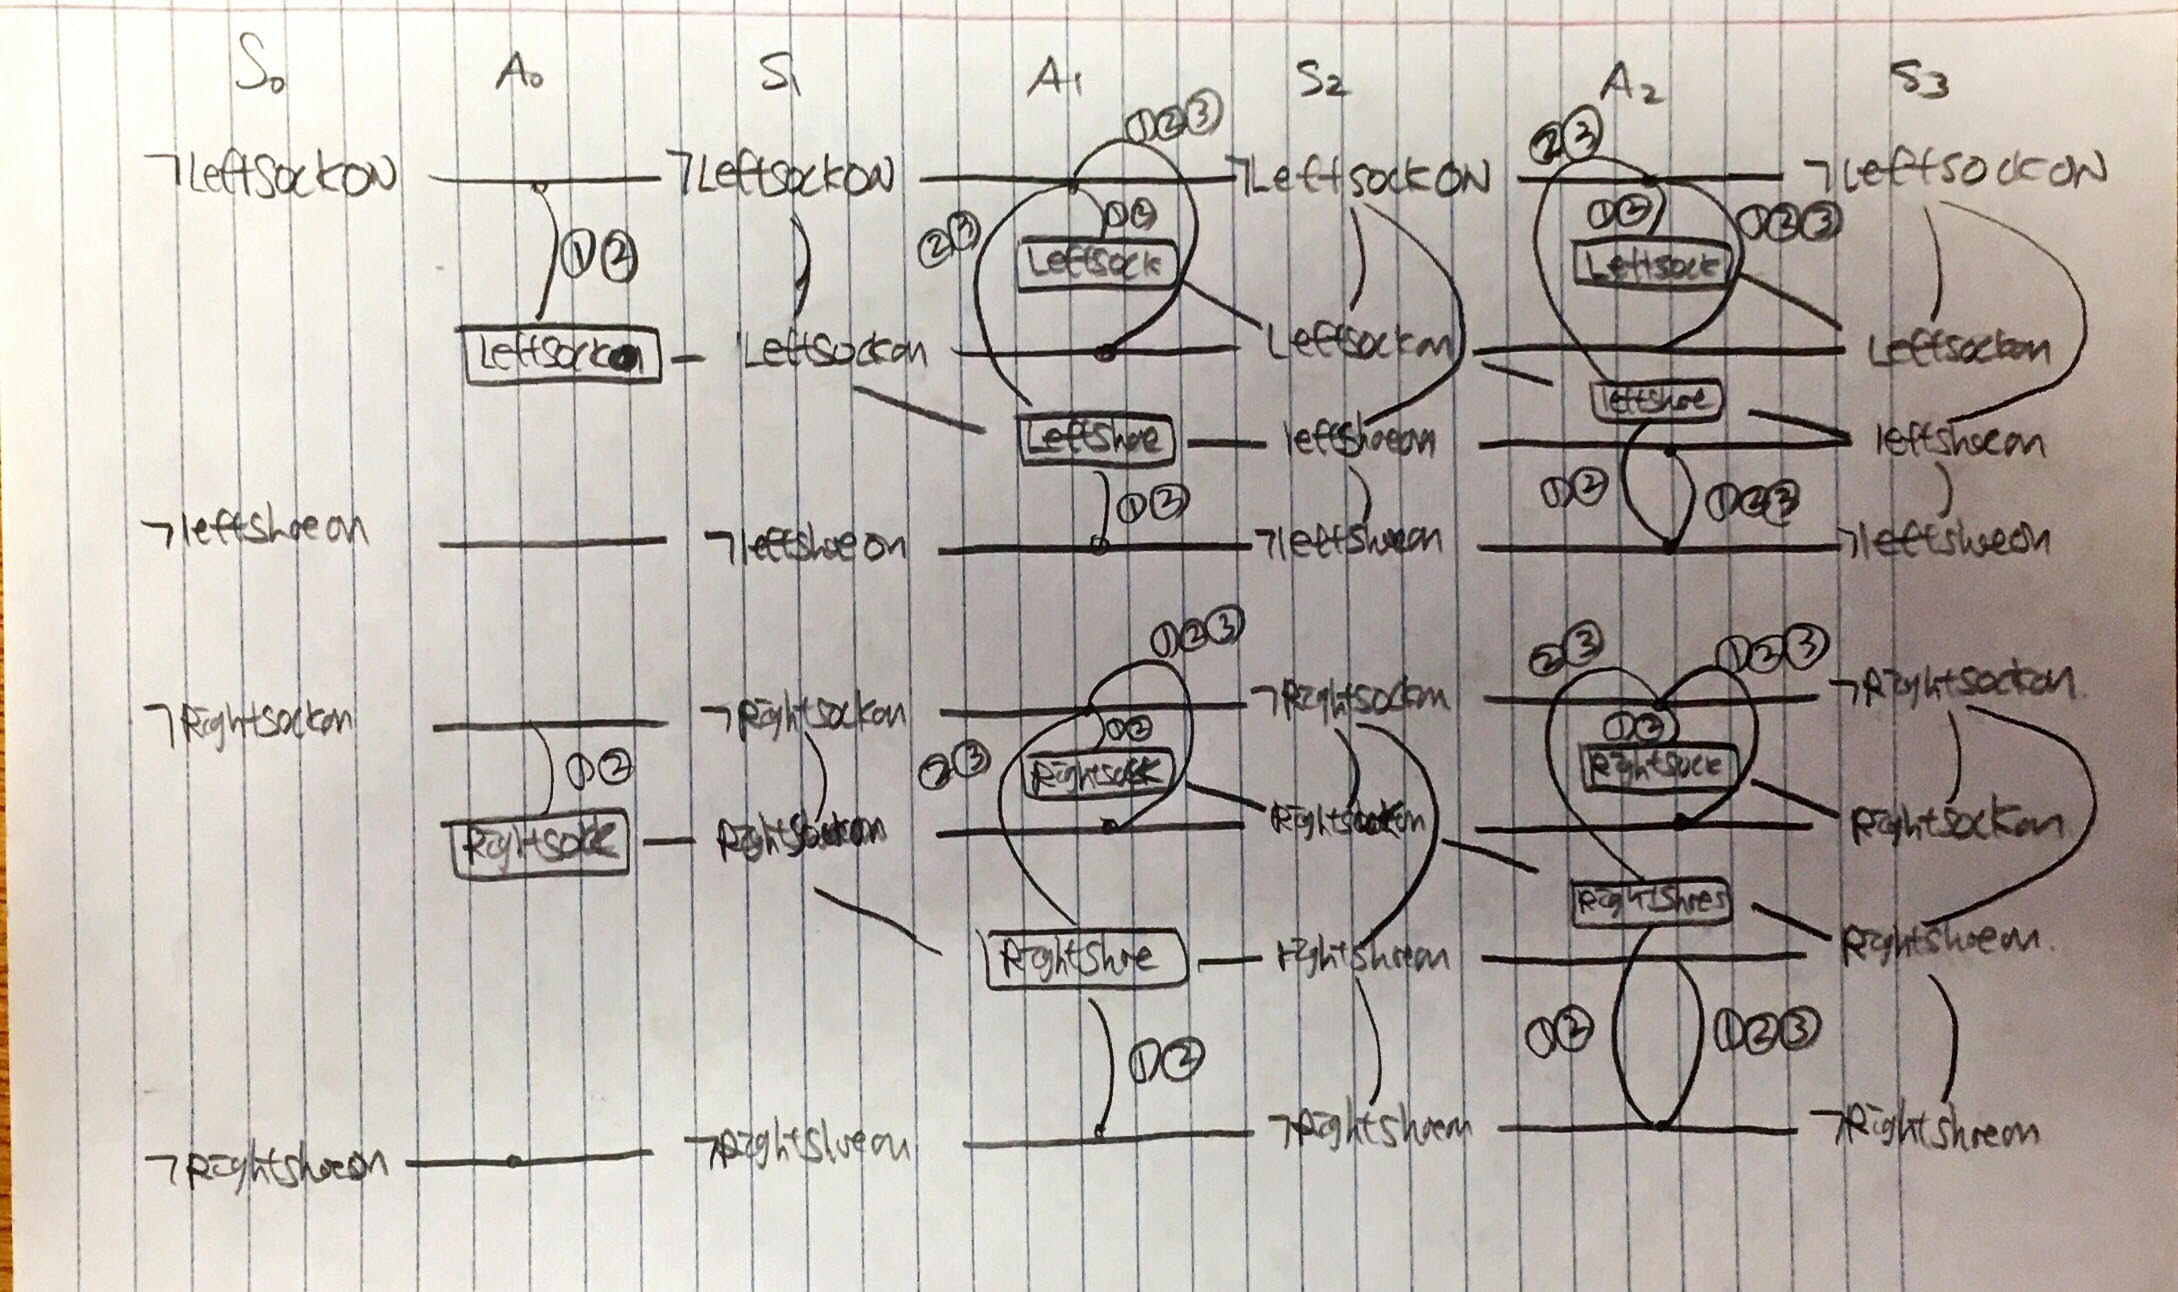
\includegraphics[width=\textwidth]{Q3.jpg}
\newline
Mutex(Actions): \newline
\newline
(1) Inconsistent \newline
(2) Interference \newline
(3) Competing needs \newline
\newline
Mutex(Literals): Inconsistent \newline
\newline
At $S_2$ and $S_3$, we can get the goal state ($RightShoeOn \wedge LeftShoeOn$). \newline
Possible Solutions: \newline
(1) $A_0$ : LeftSock, RightSock. \space $A_1$ : LeftShoe, RightShoe \newline
(2) $A_0$ : LeftSock, RightSock. \space $A_1$ : LeftShoe. \space $A_2$ : RightShoe \newline
(3) $A_0$ : LeftSock, RightSock. \space $A_1$ : RightShoe \space $A_2$ : LeftShoe \newline
(4) $A_0$ : LeftSock. \space $A_1$ : RightSock. \space $A_2$ : Leftshoe, RightShoe \newline
(5) $A_0$ : RightSock. \space $A_1$ : LeftSock. \space $A_2$ : LeftShoe, RIghtShoe \newline
\item 
\begin{enumerate}
\item How does the closed world assumption affect planning? Be precise. \newline
$\rightarrow$ \newline
Closed World Assumption means that unmentioned fluents are false. By using Closed World Assumption, we can only have fluents that are mentioned in the planning. Then, we don't need to explain about unmentioned ones so that actions become countable and states yielded from actions also become countable. \newline

\item Why preconditions in action schemas are conjunctions and not disjunctions? \newline
$\rightarrow$ \newline
Literals in precondition have to be true in state where action can be applied. If it is disjunction, literal can be both true and false so that we cannot say that the action is applied to the state or no. \newline

\item Why variables that appear in the effects of an action schema have to be in the preconditions? \newline
$\rightarrow$ \newline
Variables that affect action must be in precondition. Because we only consider fluents or variables mentioned in the domain. So the variables in effect have to be in precondition and effect in the state that action is applied. Then, the variables are bound to the certain state.
\item Why an initial state for planning needs to have ground atoms (no variables)? \newline
$\rightarrow$ \newline
An initial state for planning needs to have ground atoms. Because it is closed world and it needs to be specified to certain objects in closed world. If there are variables, they might have objects that are not specified and unbound. So it has to be no variables.
\end{enumerate}

\end{enumerate}

\end{document}
